\subsection{Evaluation the forecasting performance}
In that section, we first evaluate the quality of the forecasting step and compare it the the theoretical results provided by Theorem~\ref{th:error}. The level of the forecasting error one depends on at least two parameters:
\begin{itemize}
\item The noise variance $\sigma^2$.
\item The size of the training dataset $K$. 
\end{itemize}
In subsections~\ref{ssse:res.sine} and~\ref{ssse:res.ahm}, we study the influence of these parameters. A comparison with the theoretical results of section~\ref{se:theoretical} is also available.

\subsubsection{Sum of sine waves}
\label{ssse:res.sine}
We proved that the linear dynamic model is sufficient to catch the dynamical behavior of signals taking the form~\eqref{eq:sum.sine}. In order to validate this theoretical result, we apply the forecasting Algorithm~\ref{alg:extension} to a large number of realizations of the random vector $\bx$ following the model~\eqref{eq:model.noise}, and such that the deterministic component $\bz$ takes the form:
\[
\bz[n]\! =\!\cos\!\left(2\pi p_1 \dfrac{n}{M} \right)\! +\! R\cos\!\left(2\pi p_2 \dfrac{n}{M} \right),\quad \!\forall n\!\in\!\{1,\ldots,N\},
\]
with $N=10^4$, $M=150$, $p_1=10$, $p_2=33$ and $R=1.4$. Besides, the additive noise is chosen to be Gaussian: $\bw\sim\cN(\bzero,\bI)$.

\paragraph{Influence of the noise variance $\sigma^2$} Here, the size of the training dataset is set to $K=450$. Then, the forecasting algorithm is run on $1000$ realizations on the discrete signal $\bx$ for three different values of $\sigma$, logarithmically spaced from $10^{-3}$ to $10^{-1}$. For each of these values, we determine the experimental bias $\mu_{xp}[N-1\ell]$ and variance $\gamma_{xp}[N-1+\ell,N-1+\ell]$ in function of the forecasting sample index $\ell$ (going from $1$ to $L=100$).

The experimental results show that the bias is neither depending on the noise variance $\sigma^2$ nor the forecasting length $\ell$. Indeed, independently of $\sigma$, we always have $\mu_{xp}[N-1+\ell]\in\left[-0.03\sigma,0.03\sigma\right]$, which is negligible with respect to the magnitude of $\bz$. This result confirms the theoretical result~\eqref{eq:mean.error}. 

On Fig.~\ref{fig:res.noise.sine}, we display the experimental variance $\gamma_{xp}[N-1+\ell,N-1+\ell]$ for each value of $\sigma$ ($+$ markers). The associated theoretical asymptotic forecasting variance~\eqref{eq:cov.error.2} is also displayed in solid line. As expected, this result highlights the fact that the forecasting variance increases linearly with respect to $\sigma^2$. More surprisingly, this result shows that the forecasting variance slightly decreases with $\ell$, what is counterintuitive. It should be noted that, contrary to what expression~\eqref{eq:cov.error.2} suggests, smaller values of $\sigma$ do not  cause a decrease of the experimental variance, but an increase. This comes from the fact that when $\sigma$ is small, the matrix $\bX\bX^T$ becomes ill-conditioned. The calculation of the forecasting matrix $\tilde\bA$ in~\eqref{eq:lse} is then strongly disturbed.
\begin{figure}
%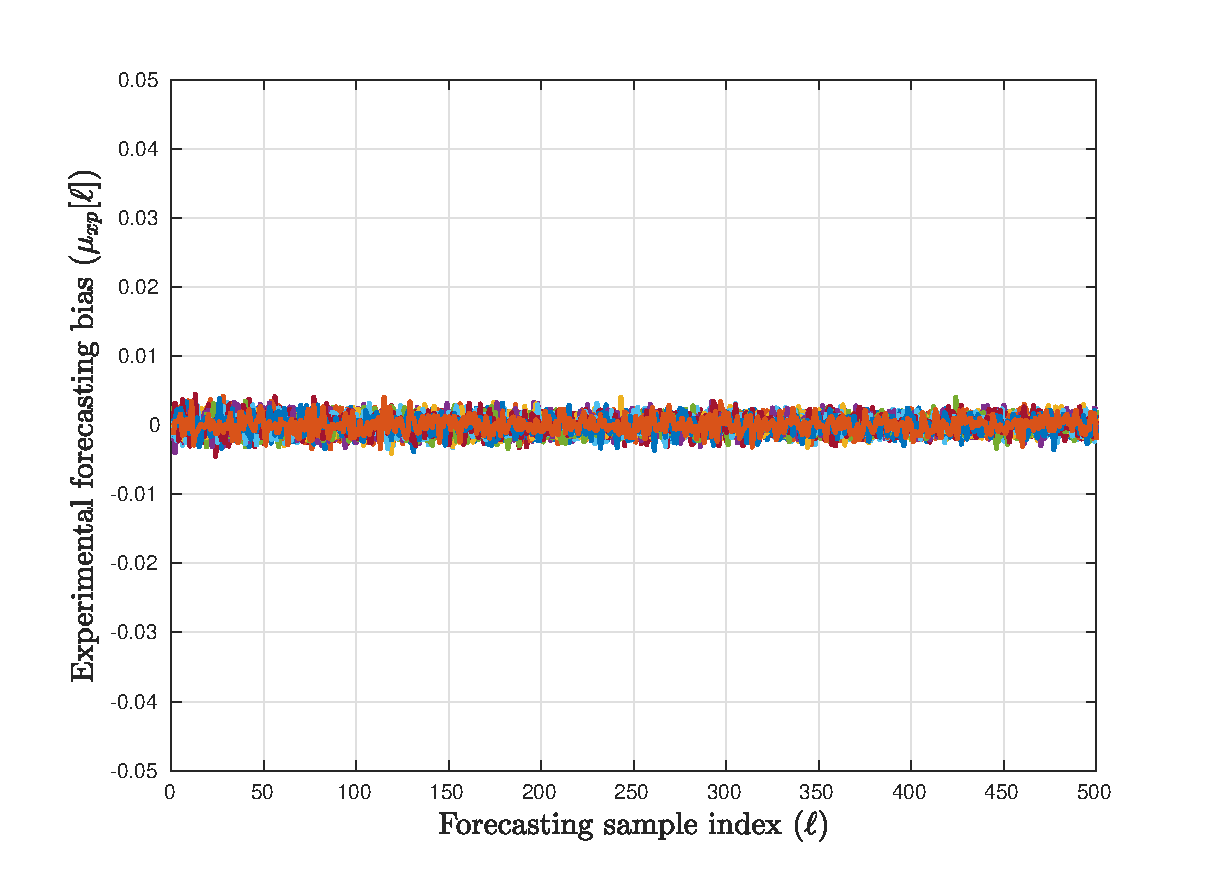
\includegraphics[width=.24\textwidth]{biasNoiseSine.eps}
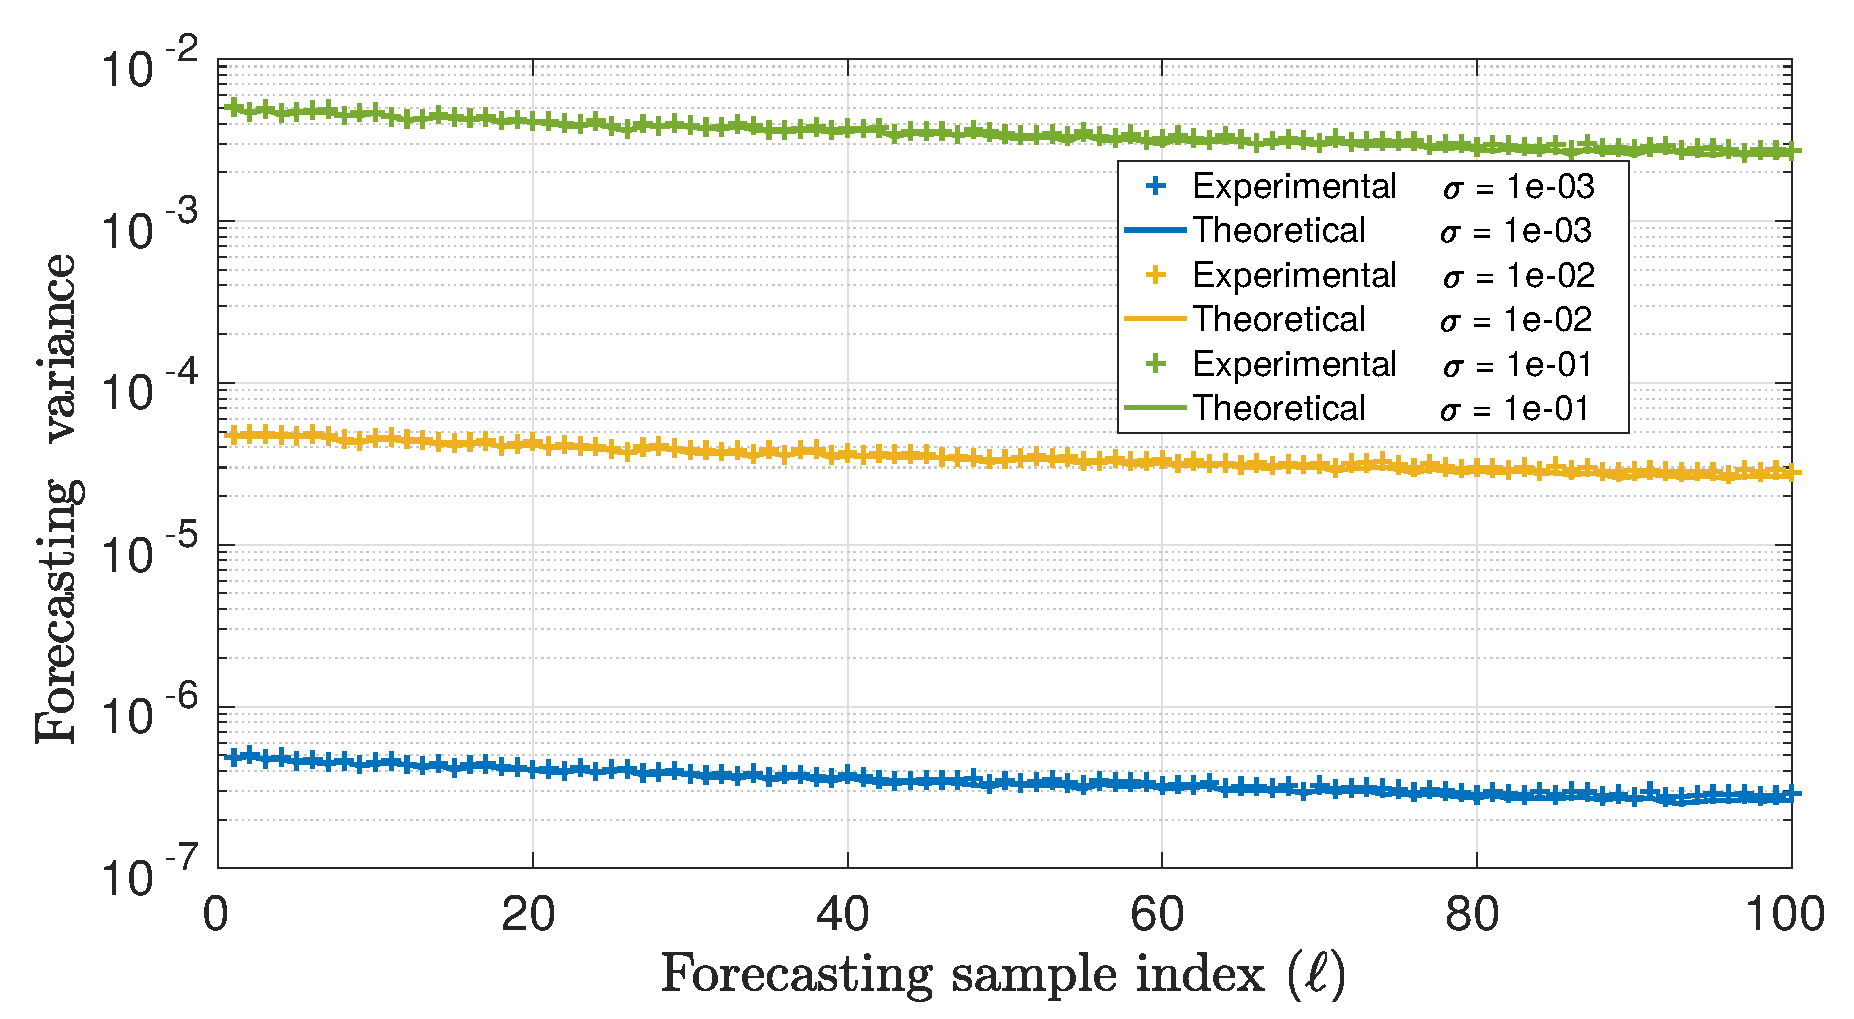
\includegraphics[width=.48\textwidth]{VarianceNoiseSine.eps}
\caption{Evolution of the experimental and theoretical forecasting variance in function of the forecasting sample index for different values of $\sigma$.}
\label{fig:res.noise.sine}
\end{figure}

\paragraph{Influence of the training dataset size $K$} Here, the noise variance $\sigma$ is set to $\sigma=10^{-2}$. Then, the forecasting algorithm is run on 3000 realizations on the discrete signal $\bx$ for three different values of $K$, logarithmically spaced from $4.5\times 10^{2}$ to $2\times 10^{3}$. For each of these values, we determine the experimental bias $\mu_{xp}[N-1+\ell]$ and variance $\gamma_{xp}[N-1+\ell,N-1+\ell]$ in function of the forecasting sample index $\ell$ (going from $1$ to $500$). 

As in the previous study, the experimental bias vanishes when $K$ increases, what confirms the approximation result~\eqref{eq:mean.error}. Besides, the experimental variance  is displayed on Fig.~\ref{fig:res.size.sine} ($+$ markers), and compared with the associated theoretical variance~\eqref{eq:cov.error.2}. Each color corresponds to these experimental results obtained for a given value of $K$. This result validates the asymptotic behavior provided by~\eqref{eq:cov.error.2}, and we can show that, as soon as $K$ is sufficiently high, the product $K\gamma[\ell,\ell]$ is approximately independent of $K$.
\begin{figure}
%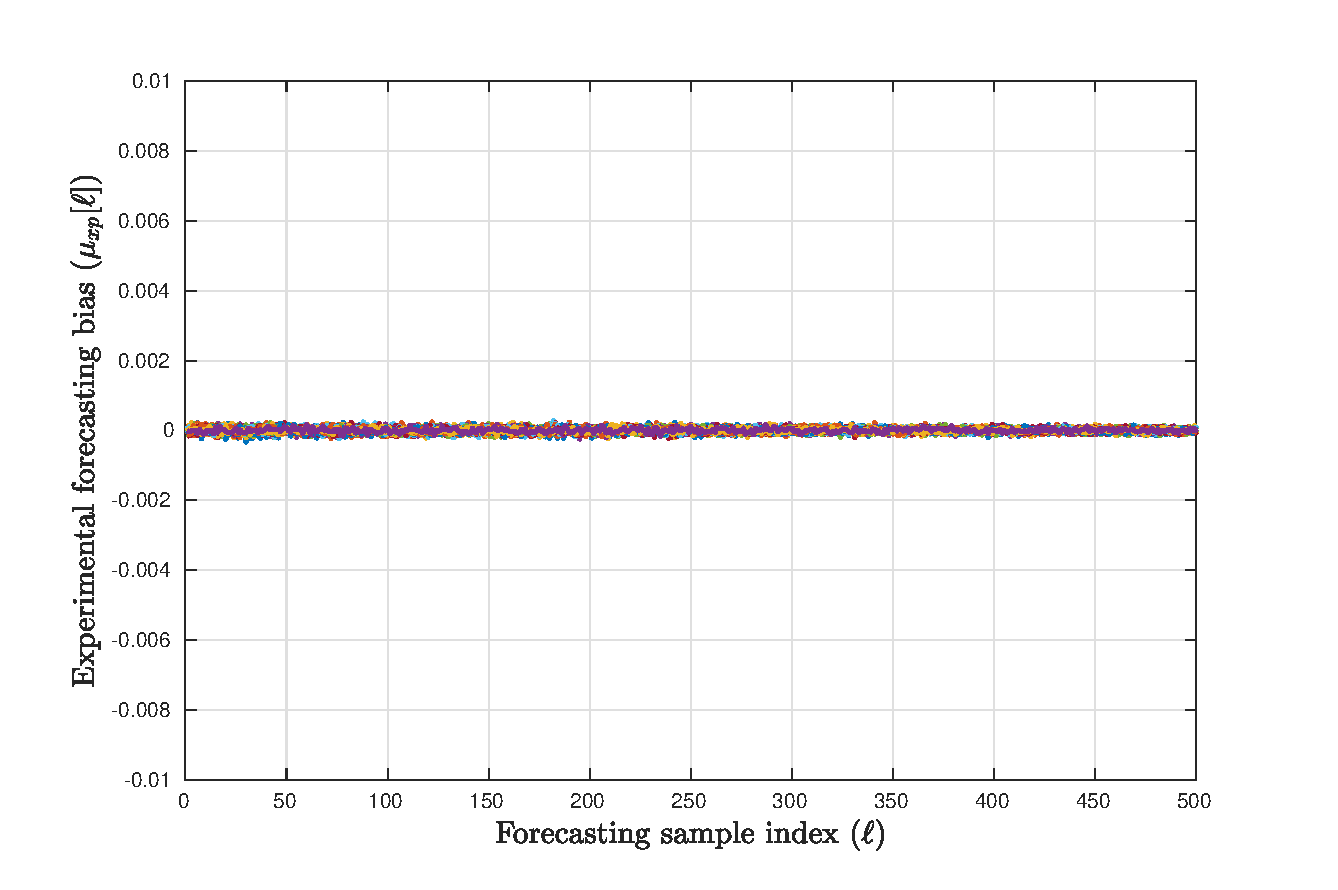
\includegraphics[width=.24\textwidth]{BiasKSine.eps}
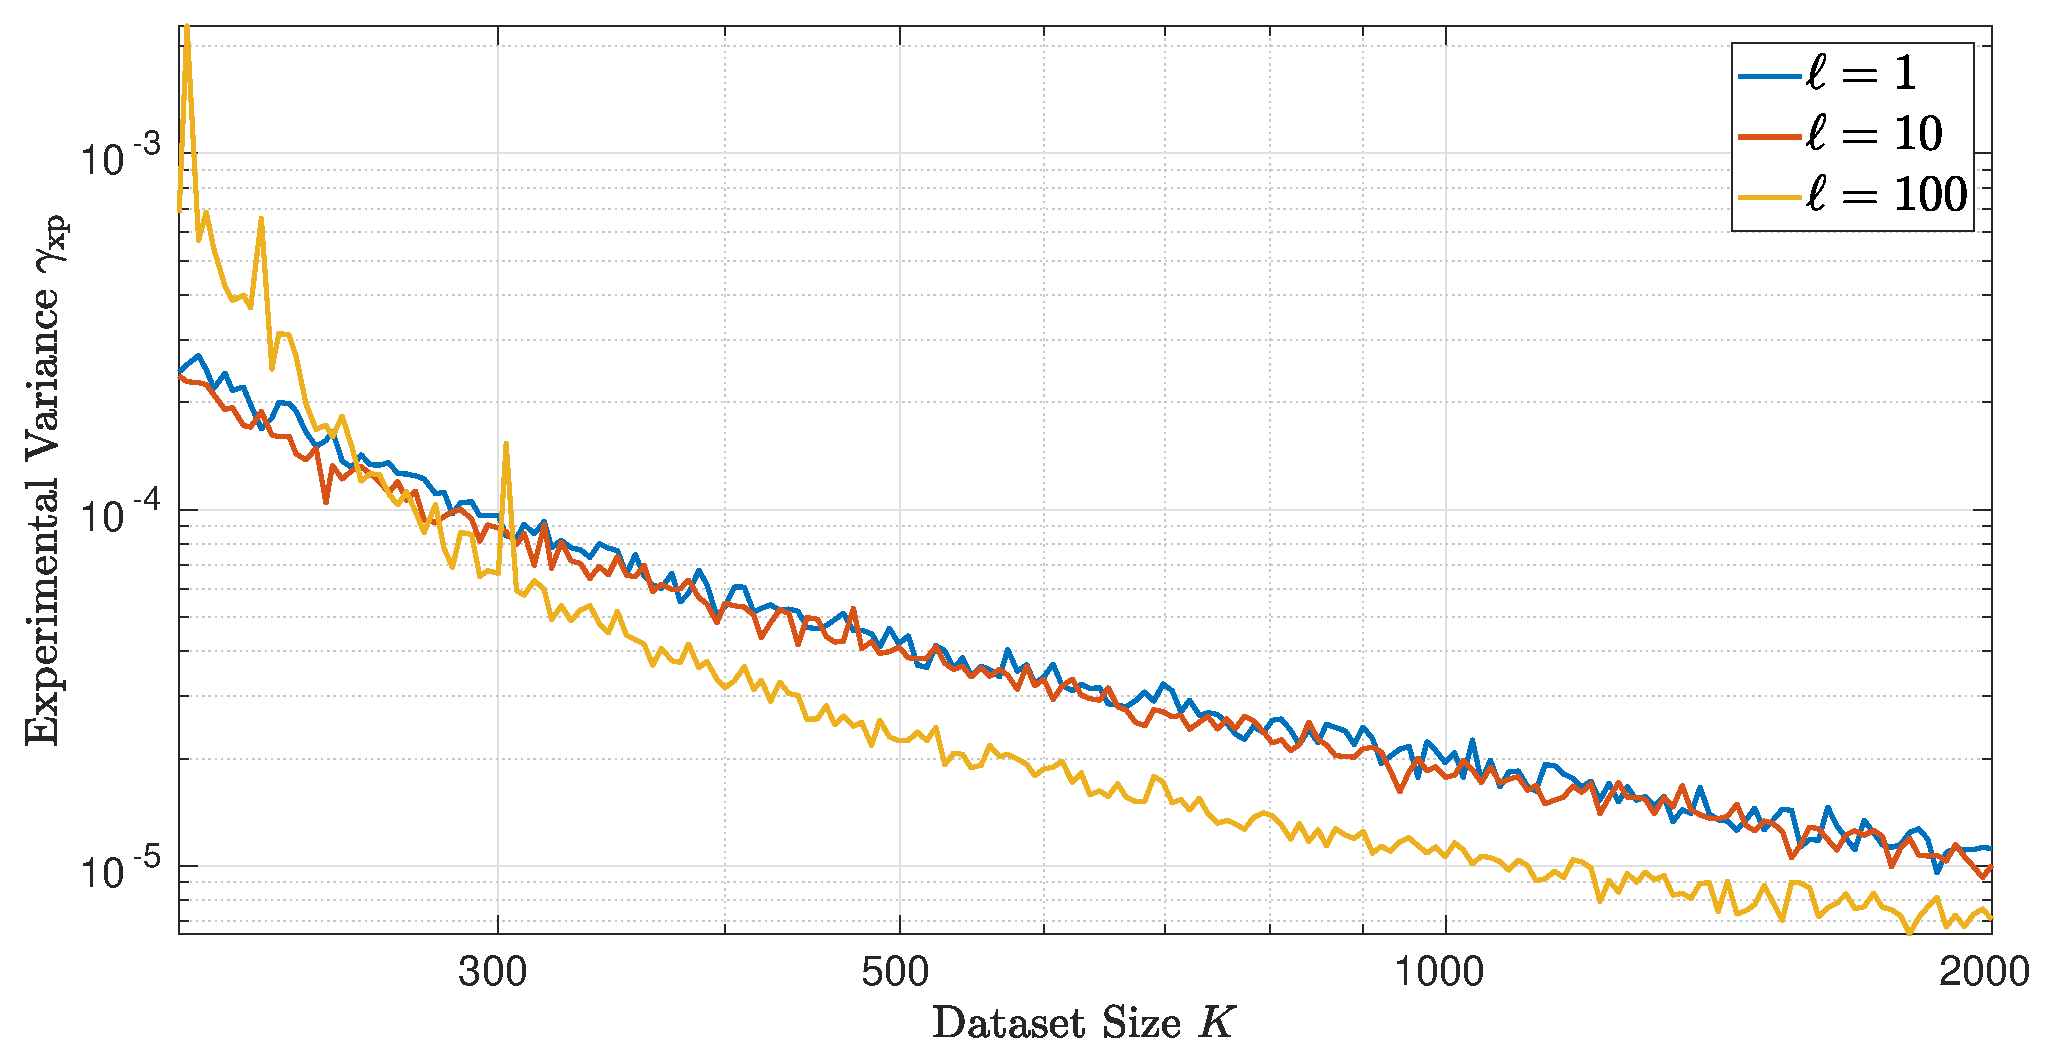
\includegraphics[width=.48\textwidth]{VarianceKSine.eps}
\caption{Evolution of the experimental and theoretical forecasting variance in function of the forecasting sample index for different values of $K$.}
\label{fig:res.size.sine}
\end{figure}

\paragraph{Summary}
Both previous experimental results combined with the theoretical asymptotic equation~\eqref{eq:cov.error.2} allow us to describe the influence of the noise variance and the size of the training dataset on the variance of the forecasting noise, which is empirically summarized as follows:
\begin{equation}
\gamma[N-1+\ell,N-1+\ell] \underset{K\to\infty}{\approx} \dfrac{\sigma^2}{K}g[\ell] .
\end{equation} 
where $g$ is a bounded positive function. The empirical result is coherent with the theoretical result provided by Theorem~\ref{th:error}.

This study neglects the analysis of the influence of the parameter $M$, whose influence on the value of the experimental variance is numerically not significant as long as $M\ll 2K$. The choice of this parameter is especially crucial when the deterministic component of the signal is no longer stationary. The adaptive harmonic model, discussed below, is an example.

\subsubsection{Adaptive harmonic model}
\label{ssse:res.ahm}
We now consider a signal whose instantaneous frequencies and amplitudes of its components vary over time. The deterministic component $\bz$ of the random vector $\bx$ ( constructed following the model~\eqref{eq:model.noise}) takes the following form, for all $n\in\{1,\ldots,N\}$:
\[
\bx[n] = \cos\left(2\pi \phi_1[n] \right) + R[n]\cos\left(2\pi \phi_2[n] \right) \ ,
\] 
where the instantaneous amplitude $R$ is given by:
\[
R[n] = 1.4 + 0.2\cos\left(4\pi\frac{n}{N}\right)\ ,
\]
and the instantaneous phases are such that:
\begin{align*}
\phi_1[n] &= \frac{p_1}{M}\left( n + \frac{0.01}{2\pi}\cos\left(2\pi\frac{n}{N}\right) \right) \\
\phi_2[n] & = p_2\frac{n}{M} + \frac{20}{2N\fs}n^2
\end{align*}
Besides, the additive noise is chosen to be Gaussian: $\bw\sim\cN(\bzero,\bI)$. Numerically, we take: $N=10^4$, $M=750$, $p_1=10$, $p_2=23$.

To highlight the fact that the linear dynamical model is sufficient to catch most of the dynamical behavior of signals following the AM-FM, we compare the performance of the Algorithm~\ref{alg:boundary} with reference forecasting algorithm that could be used for extending such signals. These methods are:
\begin{itemize}
\item The \emph{Extended Dynamic Mode Decomposition (EDMD)} has been developped by Williams \etal~\cite{Williams15data}. The proposed algorithm is a way to obtain an approximation of the so-called Koopman operator of the observed system, which theoretically allows to catch dynamic of nonlinear systems~\cite{Korda18linear}.
\item The \emph{Gaussian Process Regression (GPR)}~\cite{Rasmussen06gaussian} is a method relying on a probabilistic dynamical model. That one is based on the Gaussian process structure, and therefore offer more flexibility in the type of dynamic that could be modeled than the linear model~\eqref{eq:dyn.model}.
\item The \emph{Trigonometric , Box-Cox transformation, ARMA errors, Trend and Seasonal components (TBATS)} method~\cite{DeLivera11forecasting} is based on a classical decomposition of times series into a trend, a seasonal and an ARMA components, with a specific dynamic for the seasonal component. This model demands the estimation of numerous parameters and, by implication, may be slow. 
\end{itemize}

To quantify the global quality (\ie~not depending on $\ell$) of the forecasting approaches, we evaluate the Experimental Mean Square Error $\mathrm{MSE_{xp}}(\tilde\bx)$ of the forward forecast extended signals, namely:
\begin{align}
\label{eq:mse}
\mathrm{MSE_{\xp}}(\tilde\bx) &= \dfrac1{L}\|\tilde\bx -\bx^\mathrm{ext}\|^2 \\
\nonumber
&=\! \dfrac1{L}\sum_{\ell=1}^L \bmu_{\xp}[N\!-\!1\!+\!\ell]^2 \!+\! \bgamma_{\xp}[N\!-\!1\!+\!\ell,N\!-\!1\!+\!\ell] .
\end{align}
where $\bx^\mathrm{ext}$ is the ground-truth extended signal, that is: $\bx^\mathrm{ext} = \begin{pmatrix}\bx[-L] & \cdots & \bx[N-1+L] \end{pmatrix}$. Then, as long as the bias $\bmu[N-1+\ell]$ and the variance $\bgamma[N-1+\ell,N-1+\ell]$ of the forecasting estimator remain small for all $\ell$, the MSE takes small values either. Corresponding results are given in Table~\ref{tab:mse.sine}. They show that the naive extension we propose gives satisfying results, even though the other methods, more sophisticated, give MSE values that are somewhat smaller. Nevertheless, a major limit of those methods is the computing time they require, which prevent them from being used to exploit real-time data. Thus, {\sf SigExt} is the extension method that optimize the trade-off between the forecasting quality and the computing time. That is why, it is implemented in our algorithm for the reduction of boundary effects.

\begin{table}
\centering
\caption{AM-FM signal. Performance of the extension methods.}
\begin{tabular}{|c||c|c|c|}
  \hline
   \multirow{2}{*}{Algorithm} & \multicolumn{2}{c|}{MSE}  & \multirow{2}{41pt}{Computing time (sec.)} \\
   \cline{2-3} & Mean & Standard deviation & \\
   \hhline{|=#=|=|=|}
   {\sf SigExt} & $1.433\times 10^{-3}$ & $4.361\times 10^{-4}$ & $0.15$ \\
   \hline
   EDMD & $3.076\times 10^{-2}$ & $8.095\times 10^{-2}$ & $2.53$\\
   \hline
   GPR & $1.436\times 10^{-3}$ & $4.346\times 10^{-4}$ & $146.33$ \\
   \hline
   TBATS & $1.732\times 10^{-3}$ & $4.924\times 10^{-4}$ & $1837.12$ \\
   \hline
\end{tabular}
\label{tab:mse.sine}
\end{table} 


\subsection{Evaluation of the quality of the boundary effects reduction}

\subsubsection{Metrics}
The quality of the boundary effects reduction must be evaluated directly on the time-frequency representation. To that aim, we compare the obtained representation to the optimal representation $\ccF_N^\mathrm{opt}(\bx)$. The optimal representation is defined as the restriction of the representation of the ground-truth extended signal $\bx^\mathrm{ext}$. Therefore, we have:
\begin{equation*}
\ccF_N^\mathrm{opt}(\bx) = \cR\left( \ccF_{N+2L}(\bx^\mathrm{ext}) \right) \ .
\end{equation*} 

In the aim of comparing the different techniques, we use a criterion, proposed in~\cite{Daubechies16conceft}, that quantify the distance between a given time-frequency representation and the optimal one. It is built in analogy with the optimal transport distance, which enables quantifying the distance between two probability density functions. Let us generically denote a time frequency representation $\ccQ$. Then, for $t$ fixed, we consider the following pseudo-probability density function:
\begin{align}
p_\ccQ^t(\xi) &= \dfrac{|\ccQ(\xi,t)|^2}{\int_\RR |\ccQ(\nu,t)|^2\dd\nu}\ .
\label{eq:ppdf}
\end{align}
Then, at each instant $t$, we can then determine the optimal transport distance $d_{t}$ between the two pseudo densities. It is given by the $L^1$ norm of the difference between the associated distribution functions. In other words, we have:
\begin{equation*}
d_{t}(\ccQ,\ccF_0) = \int_\RR\left|\tilde P_{\ccQ}^t(\xi)-  P_{\ccF_0}^t(\xi)\right|\dd\xi\ ,
\end{equation*}
where $P_{\ccQ}^t(\xi)=\int_{-\infty}^\xi p_{\ccQ}^t(\nu)\dd\nu$ and $\tilde P_{\ccF_0}^t(\xi)=\int_{-\infty}^\xi\tilde p_{\ccF_0}^t(\nu)\dd\nu$.
Finally, the distance between the two time-frequency representations is obtained by averaging all the optimal transport distances with respect to time:
\begin{equation}
D(\ccQ,\ccF_0) = \frac1{|I|}\int_I d_{t}(\ccQ,\ccF_0)\dd t\ .
\end{equation}
The \textit{Optimal Transport Distance} (OTD) quantifies the proximity between the estimated and actual instantaneous frequencies while favouring the sparsity of the estimated time-frequency representation.

Let us evaluate the quality of the boundary effects reduction on biomedical signals.


\subsubsection{Respiratory signal}
We first consider a 50 minutes-long respiratory signal. This signal is sampled at $\fs=100$~Hz. A zoom on a small portion of the signal is displayed in Fig.~\ref{fig:tho}.

\begin{figure}
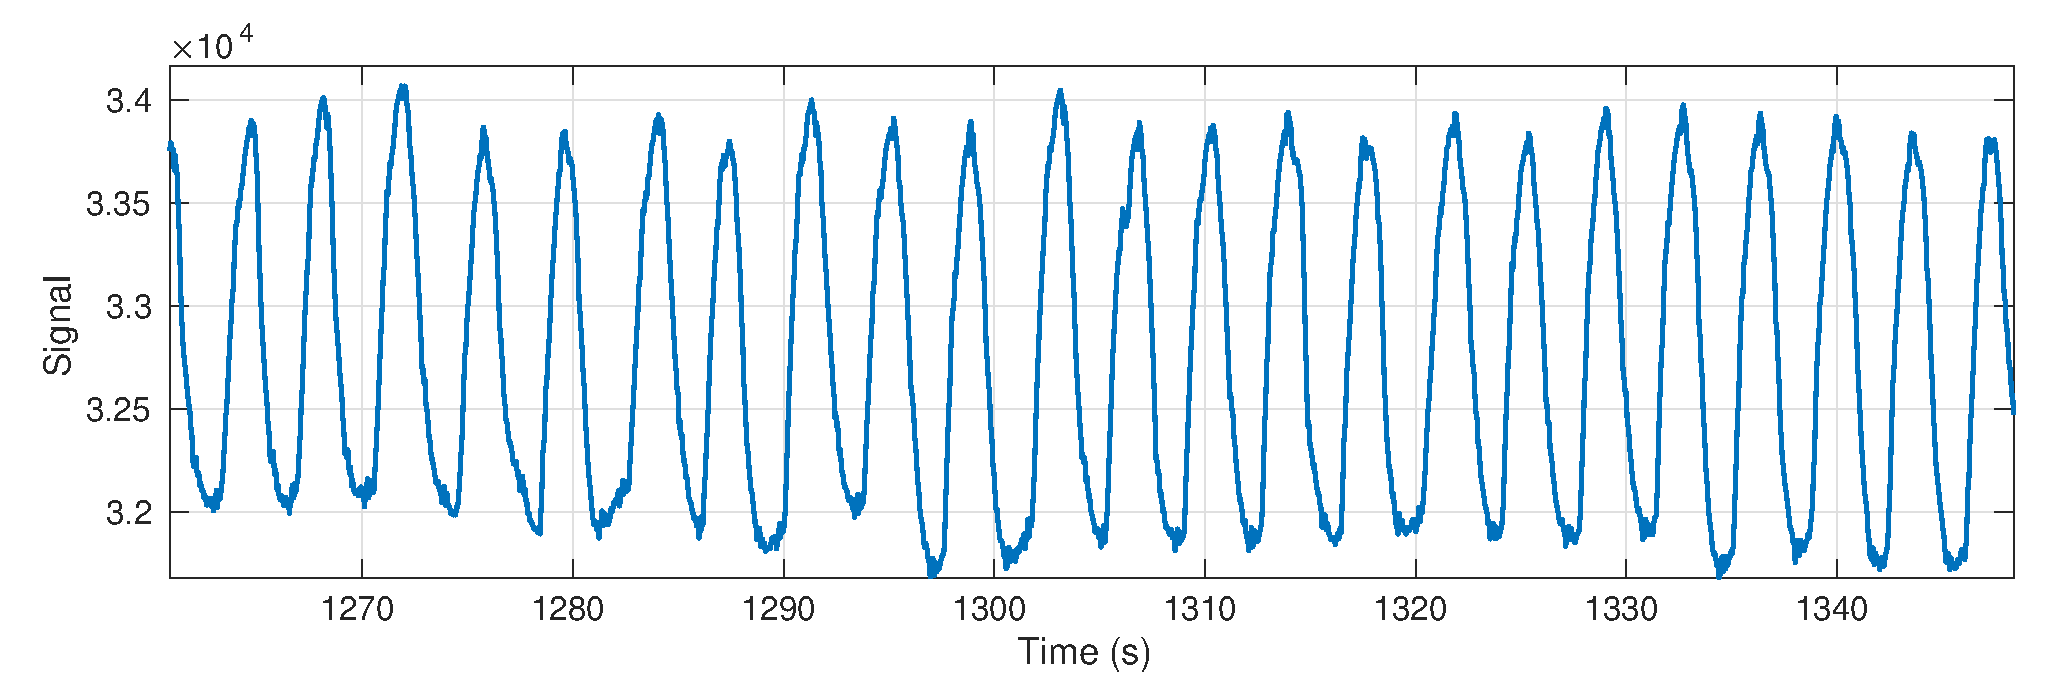
\includegraphics[width=.48\textwidth]{THOsig.eps}
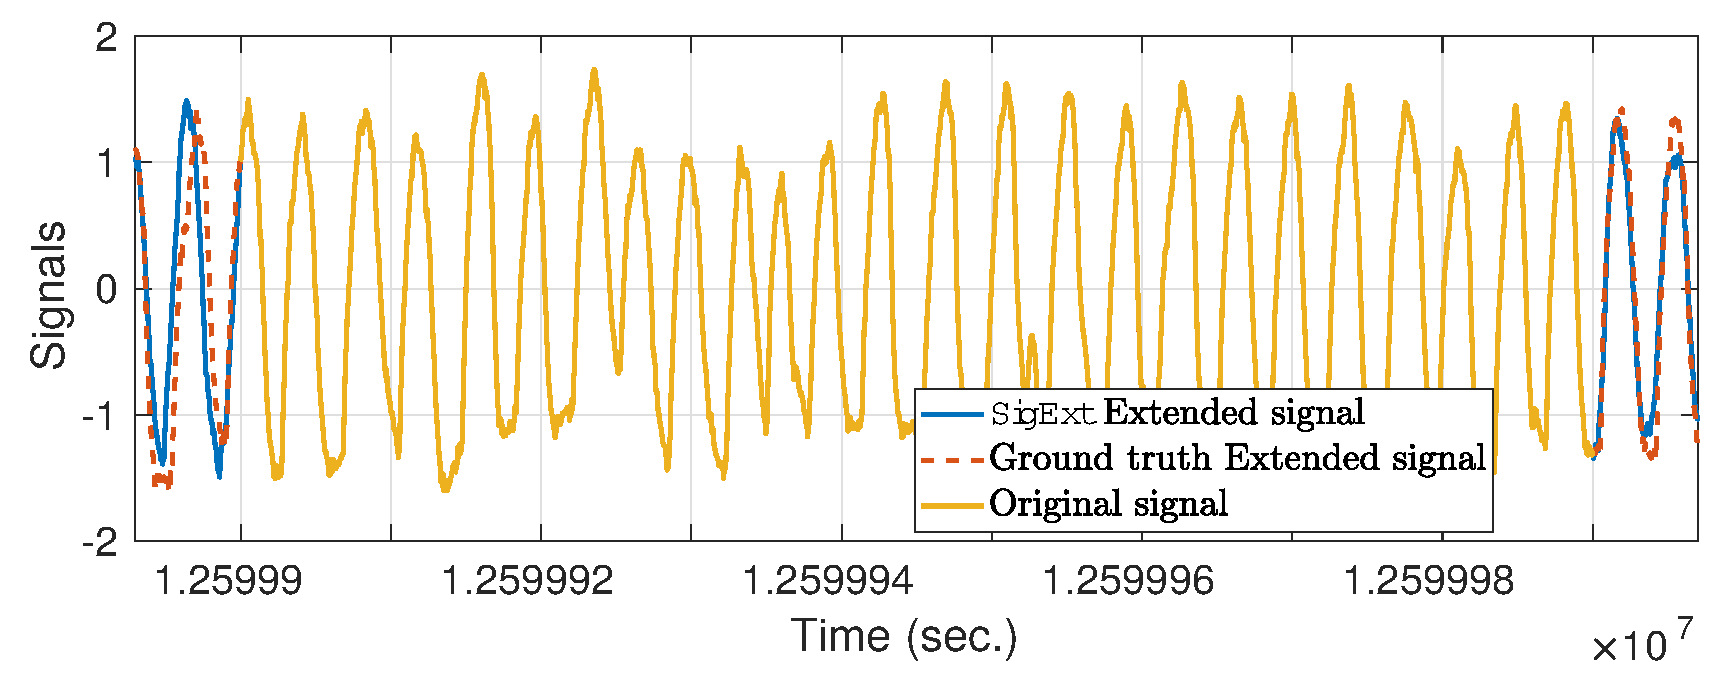
\includegraphics[width=.48\textwidth]{THOforecast.eps}
\caption{Zoom on the respiratory signal. Top: original measured signal. Extended signal obtained by {\sf SigExt} forecasting superimposed with the ground truth signal.}
\label{fig:tho}
\end{figure}

From that large signal, we build a dataset of $48$ non-overlapping signals of 60 seconds, \ie~$N=6000$. On each of these pieces of signal, we implement the forecasting method introduced in section~\ref{ssse:res.ahm}, including the {\sf SigExt} method detailed in Algorithm~\ref{alg:extension}. However, the TBATS extension method in not implemented here because of its excessive computing time. The extensions of $7$ seconds-long on each boundary, corresponding to $L =700$. Thus, in order to catch slowly varying dynamical behaviors, the size of the training signal $M$ is chosen so that $M=\lfloor 1.5L\rfloor$. As a result of section~\ref{ssse:res.sine}, we take: $K=\lfloor2.5M\rfloor$. The average and the median of the MSE~\eqref{eq:mse} with respect to the simulations are given in Table~\ref{tab:mse}. The averaged MSE of {\sf SigExt} method is overwhelmingly higher than the averaged MSE of the other methods. This result is caused by the presence of outliers in some extensions by {\sf SigExt}. Indeed, the value median of the MSE is of the same order than those of the other methods. These outliers are probably due to the presence of pulse in the respiratory signal. That ones make the AM-FM model temporarily irrelevant, and break the validity of the linear dynamical model~\eqref{eq:dyn.model} used to extend the signal. That is why {\sf SigExt} is less robust to the vanishing of oscillations that the GPR or EDMD extensions.

\begin{table}
\centering
\caption{Respiratory signal. MSE of the respiratory signal extensions.}
\begin{tabular}{|c||c|c|}
  \hline
   \multirow{2}{*}{Algorithm} & \multicolumn{2}{c|}{MSE} \\
   \cline{2-3}
      & Mean & Median\\
   \hhline{|=#=|=|}
   {\sf SigExt} & $1.704 \times 10^{1}$ & $7.346 \times 10^{-1}$ \\
   \hline
   EDMD & $2.172\times 10^{-2}$ & $7.349\times 10^{-1}$ \\
   \hline
   GPR & $4.476\times 10^{-2}$ & $1.998\times 10^{-2}$ \\
   \hline
\end{tabular}
\label{tab:mse}
\end{table} 

Then, we apply the boundary effects reduction method {\sf BoundEffRed} (Algorithm~\ref{alg:boundary}) on these extensions for diverse time-frequency representations: STFT, SST, RS, as well as ConceFT, an SST-based representation introduced in~\cite{Daubechies16conceft}. In Table~\ref{tab:otd.tho}, the results are compared in terms of OTD. They are also compared with the strategy consisting in a zero-padding extension of the signal. Even though the performance of the forecasting Algorithm~\ref{alg:extension} is somehow moderate, the boundary effects can be reduced dramatically on the time-frequency representations. Notice that the extension length $L$ has been set accordingly to the window length used by the time-frequency analysis tool. For instance, here the window length we use to evaluate the STFT is of 1500 samples. To prevent the STFT from being sensitive to the boundary effects, we set $L=750$. In this way, when evaluating the spectral content of the signal near its boundaries, the analysis is not limited by a lack of information all along the window support. From now on, all results are given for $L$ at equal to the half of the width of the window used in the time-frequency transform.  

\begin{table}
\centering
\caption{Respiratory signal. Averaged OTD of the boundary effects reduction methods on diverse representations.}
\begin{tabular}{|>{\centering}m{35pt}||c|c|c|c|}
  \hline
   \multirow{2}{35pt}{\centering Extension method} & \multicolumn{4}{c|}{Time-Frequency Representation} \\
   \cline{2-5}
      & STFT & SST & RS & ConceFT \\
   \hhline{|=#=|=|=|=|}
   Without extension & $2.16\!\times\! 10^{-2}$ & $5.26\!\times\! 10^{-3}$ & $3.07\!\times\! 10^{-2}$ & $1.41\!\times\! 10^{-2}$ \\
   \hline
   {\sf SigExt} & $1.72\!\times\! 10^{-2}$ & $4.00\!\times\! 10^{-3}$ & $2.43\!\times\! 10^{-2}$ & $1.12\!\times\! 10^{-2}$ \\
   \hline
   EDMD & $1.75\!\times\! 10^{-2}$ & $4.23\!\times\! 10^{-3}$ & $2.45\!\times\! 10^{-2}$ & $1.09\!\times\! 10^{-2}$ \\
   \hline
   GPR & $1.84\!\times\! 10^{-2}$ & $4.10\!\times\! 10^{-3}$ & $2.48\!\times\! 10^{-2}$ & $1.24\!\times\! 10^{-2}$ \\
   \hline
\end{tabular}
\label{tab:otd.tho}
\end{table}


\subsubsection{Photoplethysmogram}
\label{ssse:ppg}
We perform a study similar to the previous one on a 640 second-long photoplethysmogram (PPG) signal, sampled at $\fs=125$~Hz. A 32 second-long piece of this signal is displayed on the top of Fig.~\ref{fig:ppg}. The estimated 2-second extension obtained by {\sf SigExt} on both boundary of this signal is superimposed to the ground-truth signal in the bottom of Fig.~\ref{fig:ppg}.

\begin{figure}
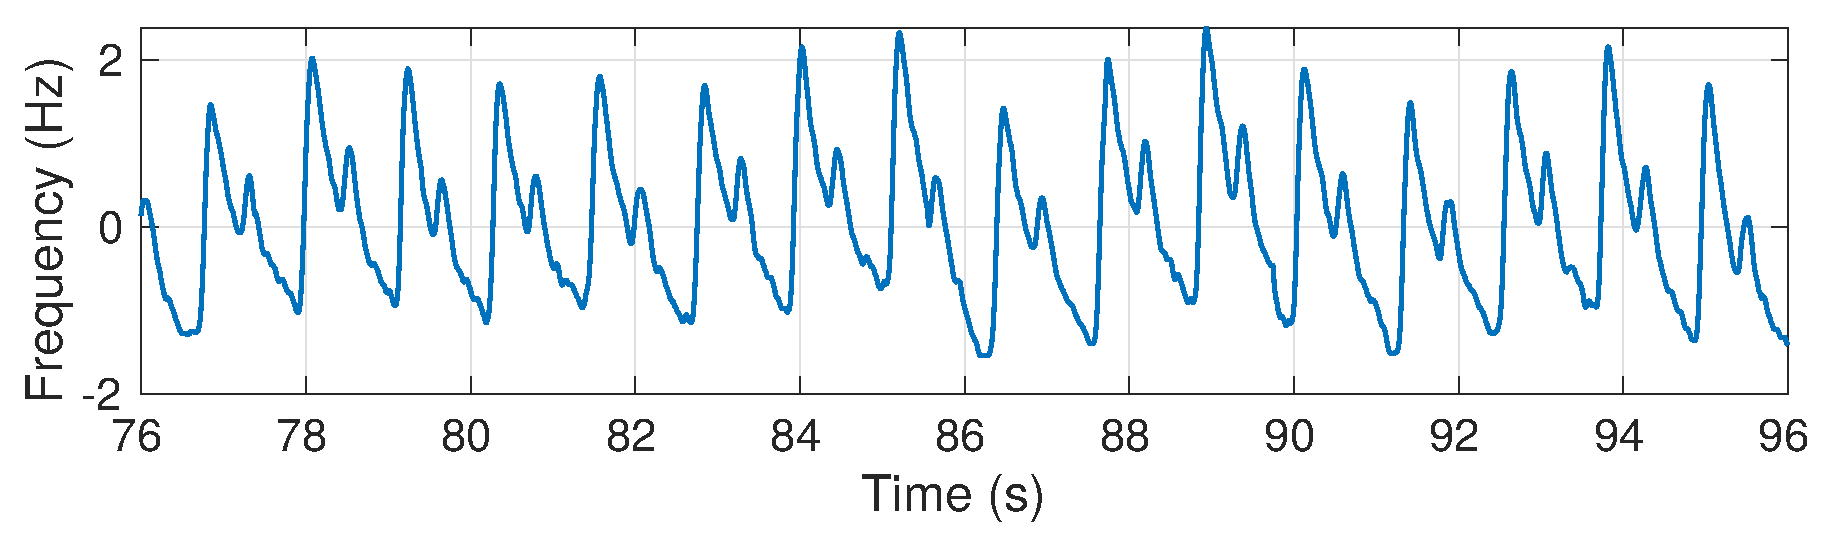
\includegraphics[width=.48\textwidth]{PPGsig.eps}
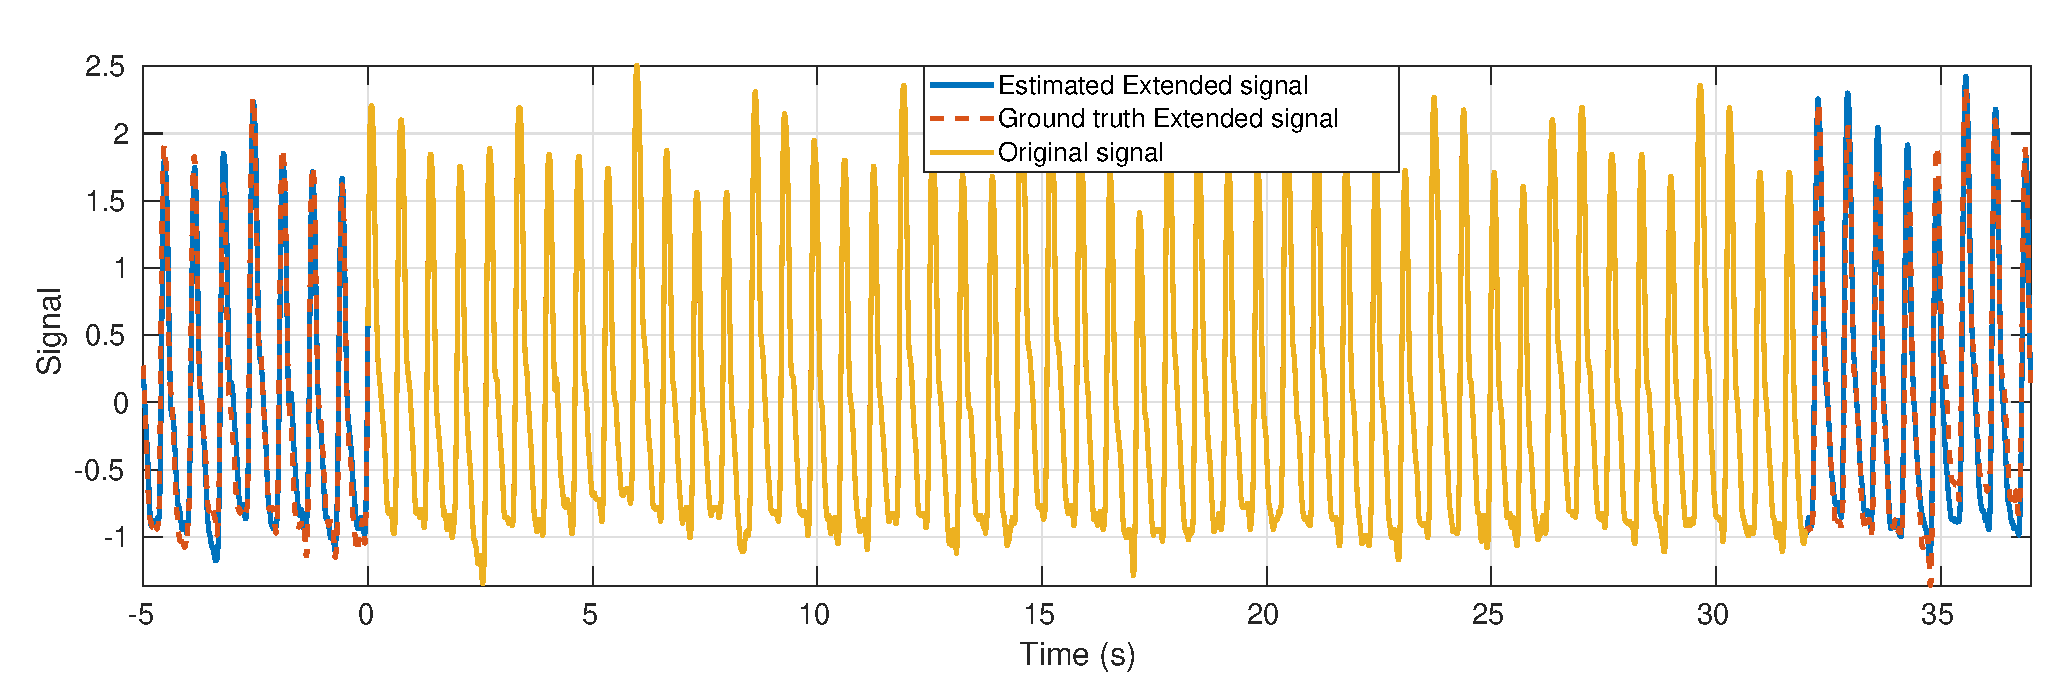
\includegraphics[width=.48\textwidth]{PPGforecast.eps}
\caption{PPG signal. Top: original measured signal. Extended signal obtained by forecasting superimposed with the ground truth signal.}
\label{fig:ppg}
\end{figure}

We divide the signal into 32-second long pieces, and apply Algorithm~\ref{alg:boundary} on each piece. We provide in Table~\ref{tab:otd.ppg} the OTD to the optimal time-frequency representation averaged over the signals. For all the considered time-frequency representations, the results clearly shows that our algorithm reduce the influence of the boundary effects. This highlights the ability of our approach to limit the distortion due the boundary effects and provide a more accurate representations. Even though the {\sc SigExt} extension yields time-frequency  representations slightly more sensitive to boundary effects that the extensions given by EDMD or GPR, it is the only technique that allows a real-time implementation.

\begin{table}
\centering
\caption{PPG signal. Averaged OTD of the boundary effects reduction methods on diverse representations.}
\begin{tabular}{|c||c|c|c|}
  \hline
   \multirow{2}{*}{Extension method} & \multicolumn{3}{c|}{Time-Frequency Representation} \\
   \cline{2-4}
      & STFT & SST & RS\\
   \hhline{|=#=|=|=|}
   Without extension & $2.52\times 10^{-2}$ & $9.41\times 10^{-2}$ & $1.03\times 10^{-1}$ \\
   \hline
   {\sf SigExt} & $1.22\times 10^{-3}$ & $7.31\times 10^{-2}$ & $1.11\times 10^{-1}$ \\
   \hline
   EDMD & $9.83\times 10^{-4}$ & $5.59\times 10^{-2}$ & $9.80\times 10^{-2}$ \\
   \hline
   GPR & $1.14\times 10^{-3}$ & $7.02\times 10^{-2}$ & $1.07\times 10^{-1}$ \\
   \hline
\end{tabular}
\label{tab:otd.ppg}
\end{table}

On Fig.~\ref{fig:ppg.boundeffred}, we display the SST resulting from the {\sf BoundEffRed} strategy, applied to the same portion of PPG than what is used to display Fig.~\ref{fig:ppg}. We clearly observe an improvement of the quality of the SST near boundaries. Indeed, the blurring visible when zooming on the right boundary of the SST has almost vanished (see bottom of Fig.~\ref{fig:ppg.boundeffred}). The real-time tracking of the instantaneous frequencies contained in the measured signal is therefore largely facilitated.

\begin{figure}
\centering
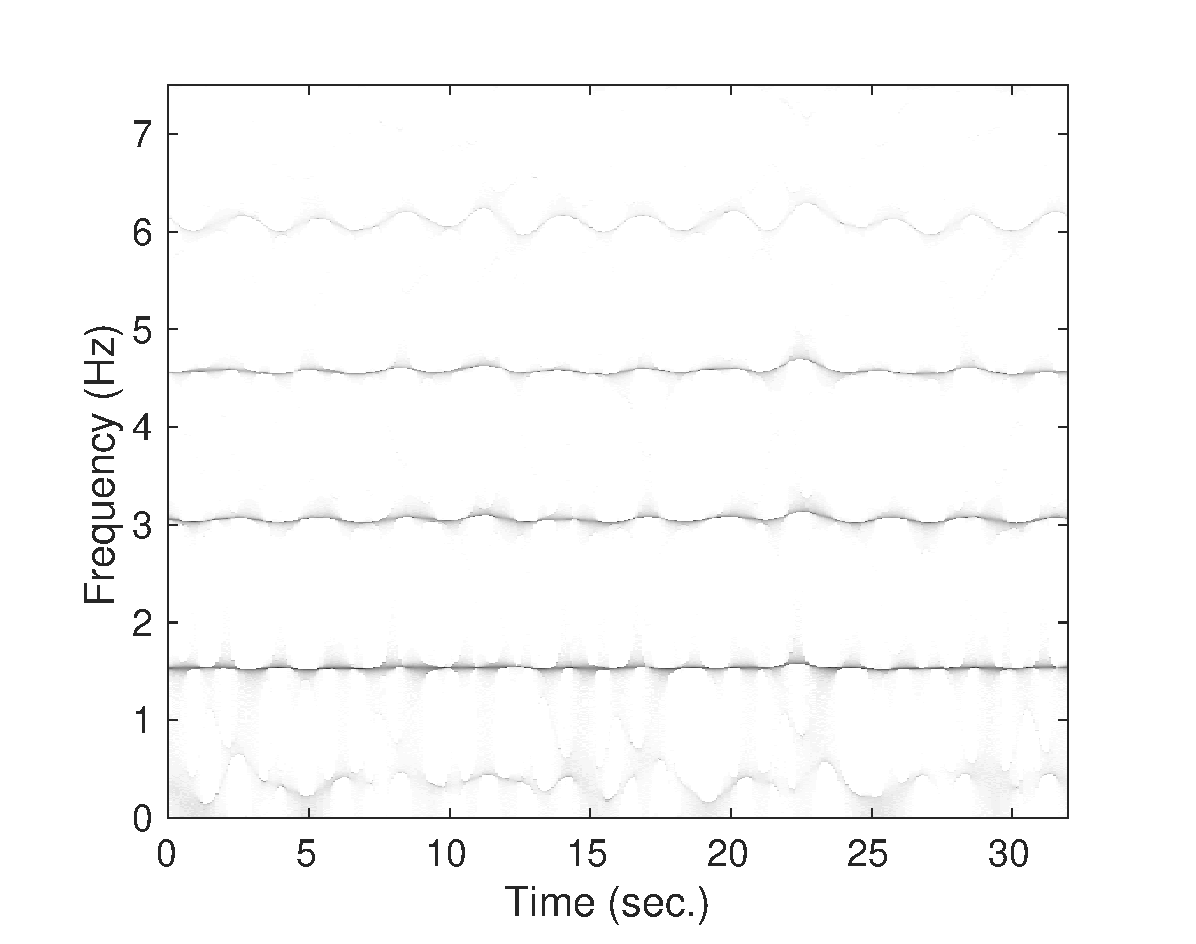
\includegraphics[width=.48\textwidth]{SSTBoundEffRed.eps}
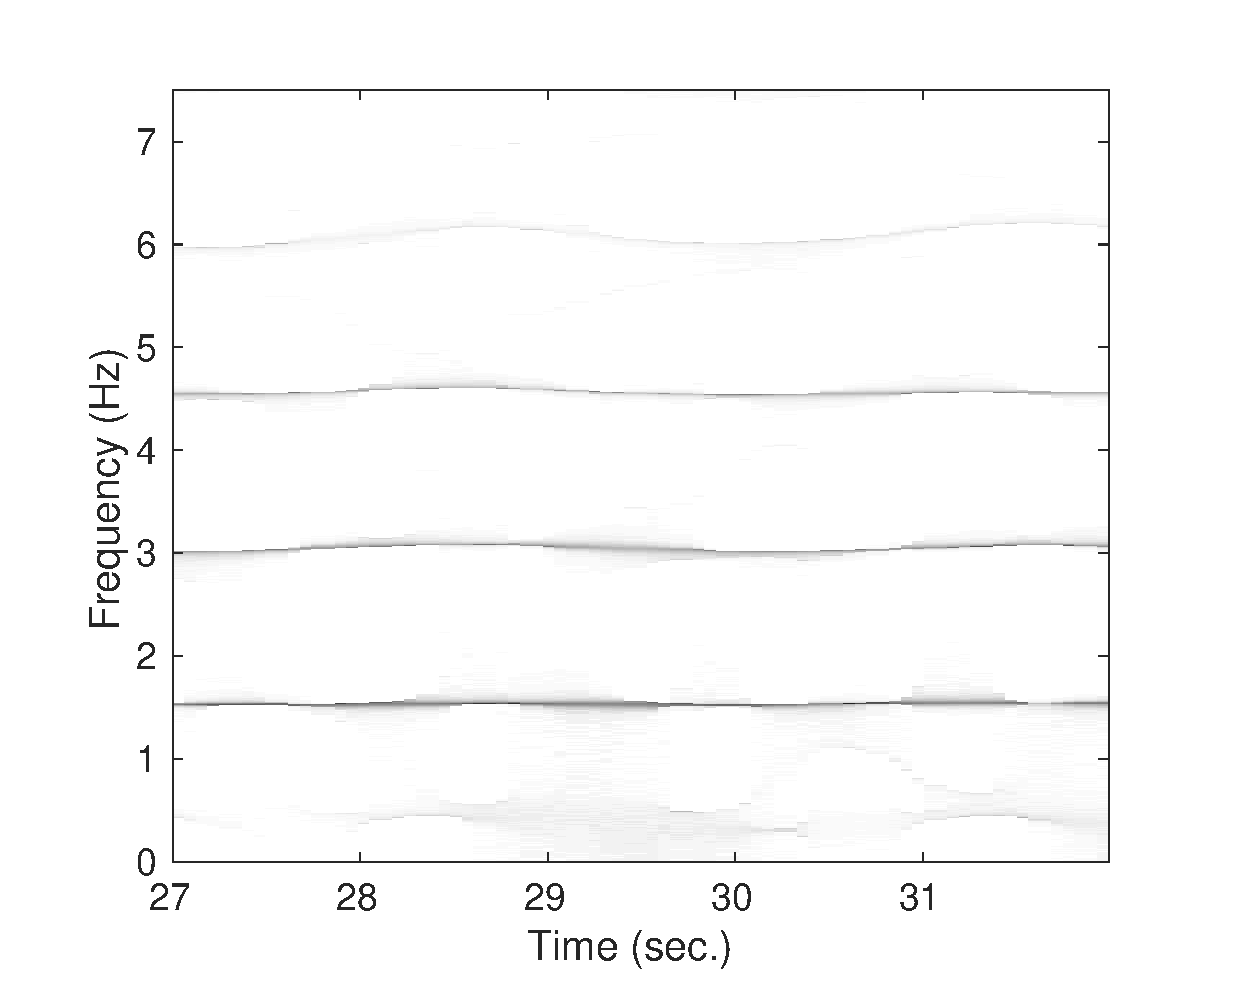
\includegraphics[width=.48\textwidth]{zoomSSTBoundEffRed.eps}
\caption{Result of {\sf BoundEffRed} on the synchrosqueezing transform of a PPG (top) with a zoom on its right boundary (bottom). }
\label{fig:ppg.boundeffred}
\end{figure}


To evaluate the influence of the noise level on the performance of {\sf BoundEffRed}, we artificially add a Gaussian noise to the measured PPG signal, whose variance is denoted $\sigma_{\mathrm{add}}^2$. It is thus an additional noise to the measurement noise actually contained in the signal. Fig.~\ref{fig:otd.noise} shows the averaged OTD of {\sf BoundEffRed} for different values of $\sigma_{\mathrm{add}}^2$. At first glance, we notice that STFT is slightly more sensitive to noise than SST or RS. On one hand, the robustness to noise of the SST and the RS is the direct consequence of the approximation result of~\cite{Daubechies16conceft}, discussed in section~\ref{sse:perf.BoundEffRed}. On the other hand, the sentivity to noise of the STFT may be interpreted as the inability to forecast the values of the time-frequency coefficients where only noise is active, while sharp time-frequency representations, such as SST or RS, ideally vanish at these points.
\begin{figure}
\centering
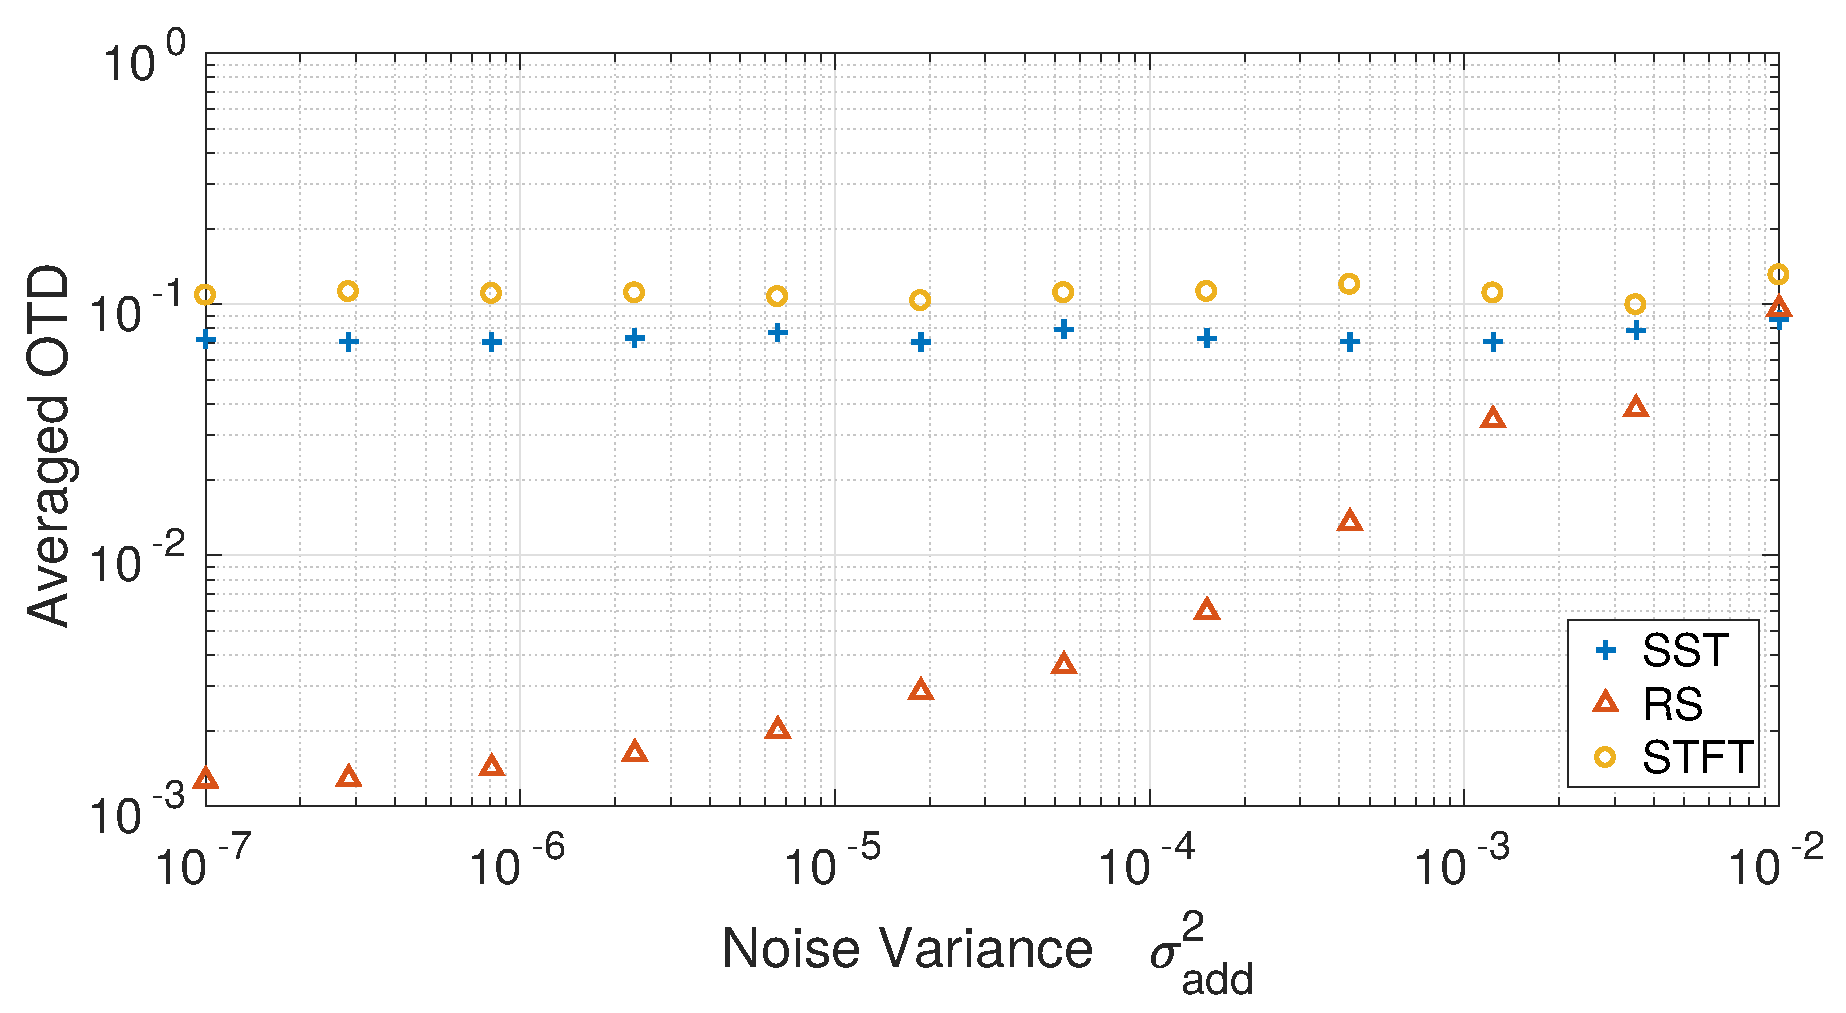
\includegraphics[width=.48\textwidth]{OTDBoundEffRed.eps}
\caption{PPG signal. Averaged OTD of {\sf BoundEffRed} in function of the noise variance.}
\label{fig:otd.noise}
\end{figure} 